The door node is the hardware that will be located at each door. It consists of
a NFC security badge reader, infrared temperature sensor, time of flight range
sensor and elextronic door lock, all connected to a Raspberry Pi.

Figure \ref{fig:door-node-schematic} shows a schematic of the door node.

\begin{figure}[!htb]
\centering
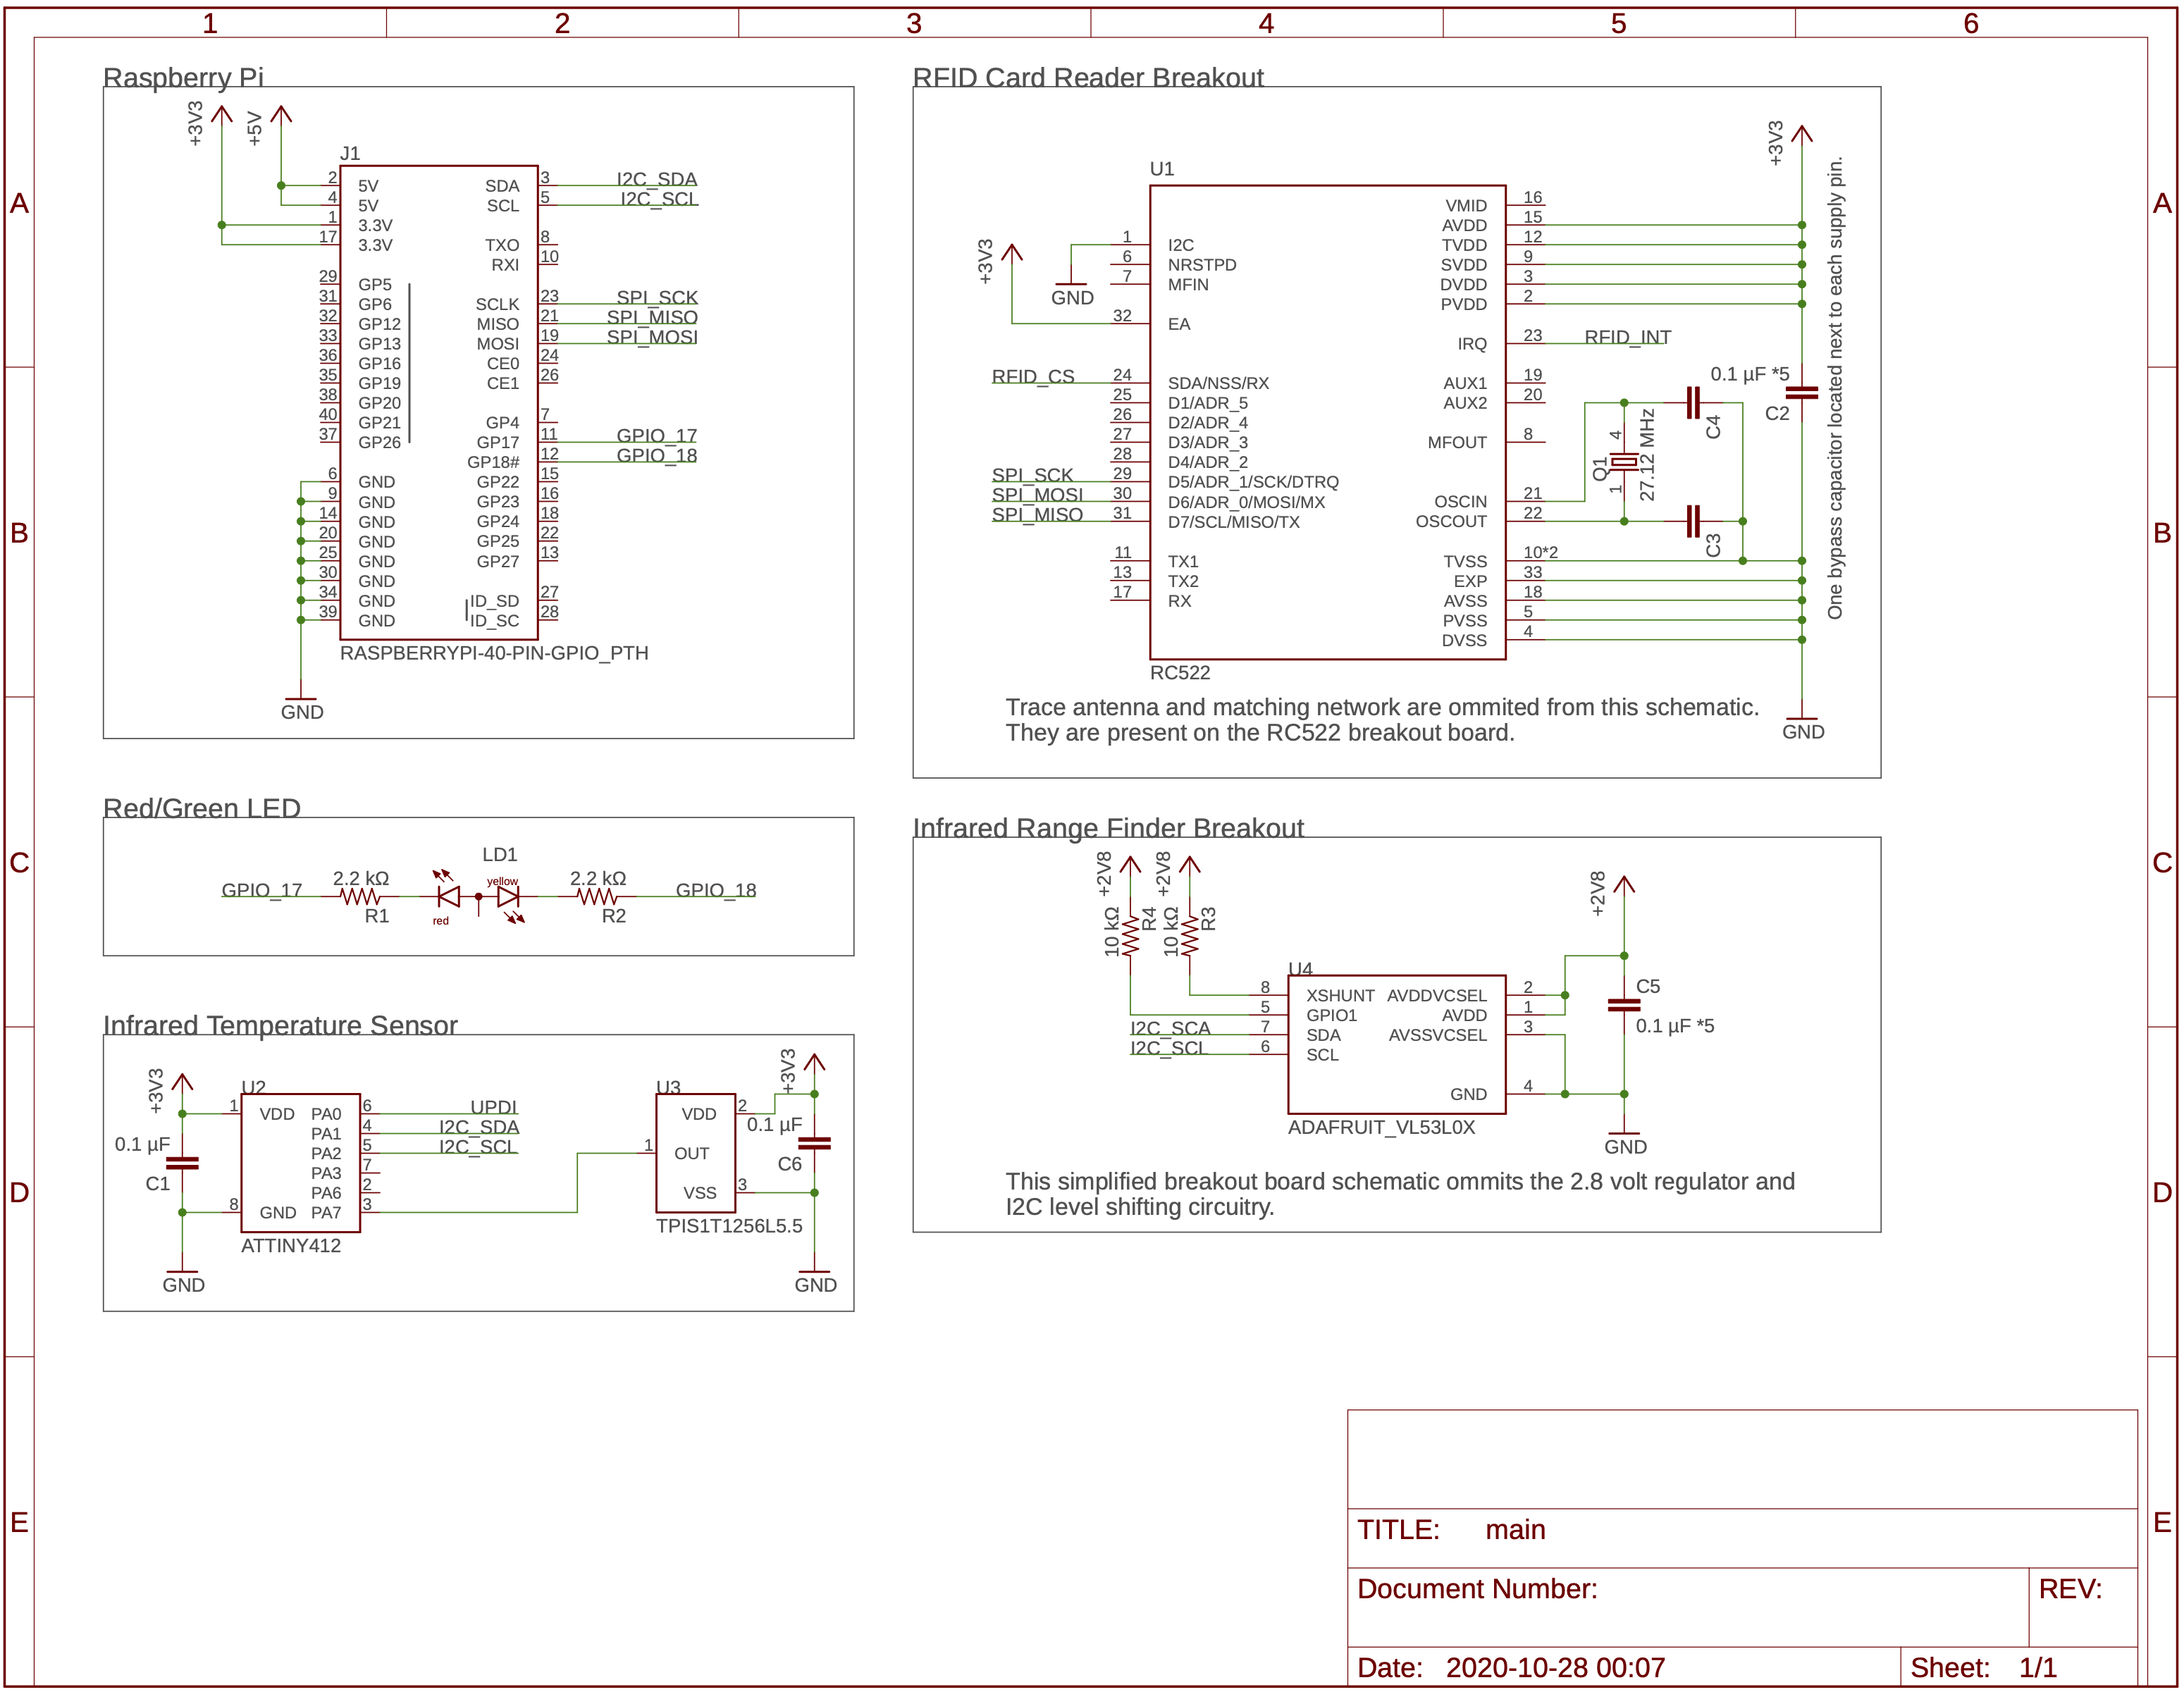
\includegraphics[width=\textwidth]{images/door-node-schematic.png}
\caption{Door Node Schematic}
\label{fig:door-node-schematic}
\end{figure}

\subsection{Infrared Temperature Sensor}

In order to detect fever we need to measure the temperature of the users of our
system. We have determined that a forehead temperature measurement using an
infrared temperature sensor is the best way to obtain sufficiently accurate
contactless temperature measurements.

We plan to use the TPiS 1T 1256 L5.5 thermopile from Excelitas Technologies.
This temperature sensor was chosen after a comparison of available infrared
temperature sensors.

The TPiS 1T 1256 L5.5 offers medical grade accuracy within the temperature range
expected for human skin. It also provides accurate ambient temperature
measurments. The optics of the sensor provide a relativly narrow 5 degree field
of view which is appropriate for measuring the fairly small target of a human
forehead from a reasonable range.

The TPiS 1T 1256 L5.5 can be powered from the Raspberry Pi's 3.3 volt rail and
features a single pin digital interface of readout of the temperature data. This
digital interface requires more accruate timing than can easily be accomplished
with a Raspberry Pi so a small 8 bit microcontroller will be used with minimal
firmware that converts betweem the thermopile's digital interface and an I2C
interface.

Figture \ref{fig:ir-test-circuit} shows the test circuit for the infrared
temperature sensor.

\begin{figure}[!htb]
\centering
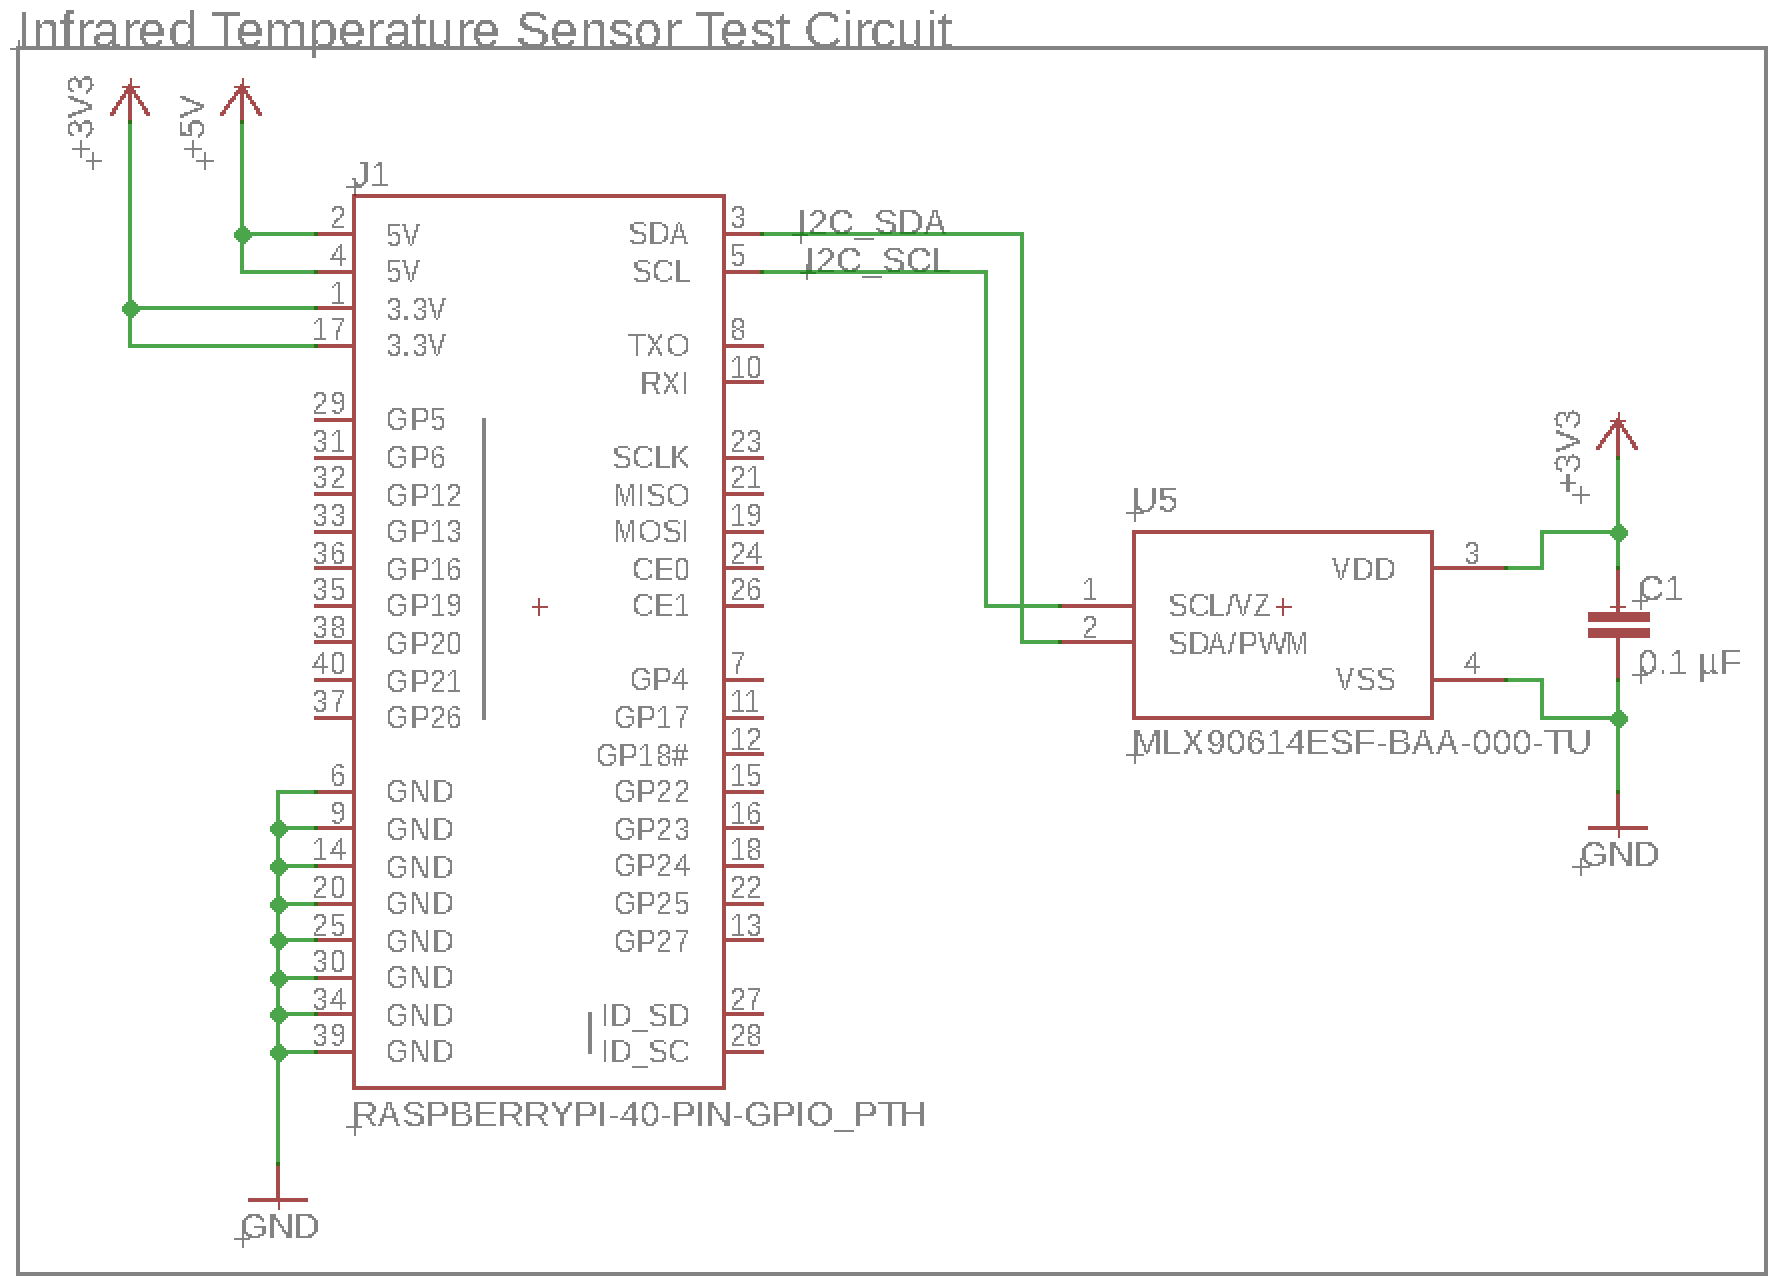
\includegraphics[width=0.75\textwidth]{images/ir-test-circuit.png}
\caption{Test Circuit for Infrared Temperature Sensor}
\label{fig:ir-test-circuit}
\end{figure}

\subsection{NFC Security Badge Reader}

The MFRC522 RFID reader is the chosen device for the NFC security badge reader. 
It has an operating distance of up to 50 mm which means that the users will not have to place
the card almost touching the reader. the fact that it includes a programmable timer
is very useful as it can help avoid creating issues where it scans a card multiple times 
when doing a single swipe. As the reader is not meant to be the end all of deciding 
whether or not an employee will unlock the door it is therefore useful that the device
supports power down by software mode. When in lockdown or an employee attempts
to enter the building at full capacity it will be powered-down preventing entrance.  
The usage of serial peripheral interface helps as the badge reader functions quickly 
being able to handle data speeds up to 10 Mbit/s. 
It is powered by the 3.3 V DC power source of the Raspberry Pi.


For the below test circuit the differences between the test circuit and the actual demo circuit
are as follows. The T GPIO extension board used is coloured differently
and indicates GPIO rather than "\#" before the numbers. 
Other then those two changes the below circuit is identical to that which will be used in demonstrations.

\begin{figure}[!htb]
\centering
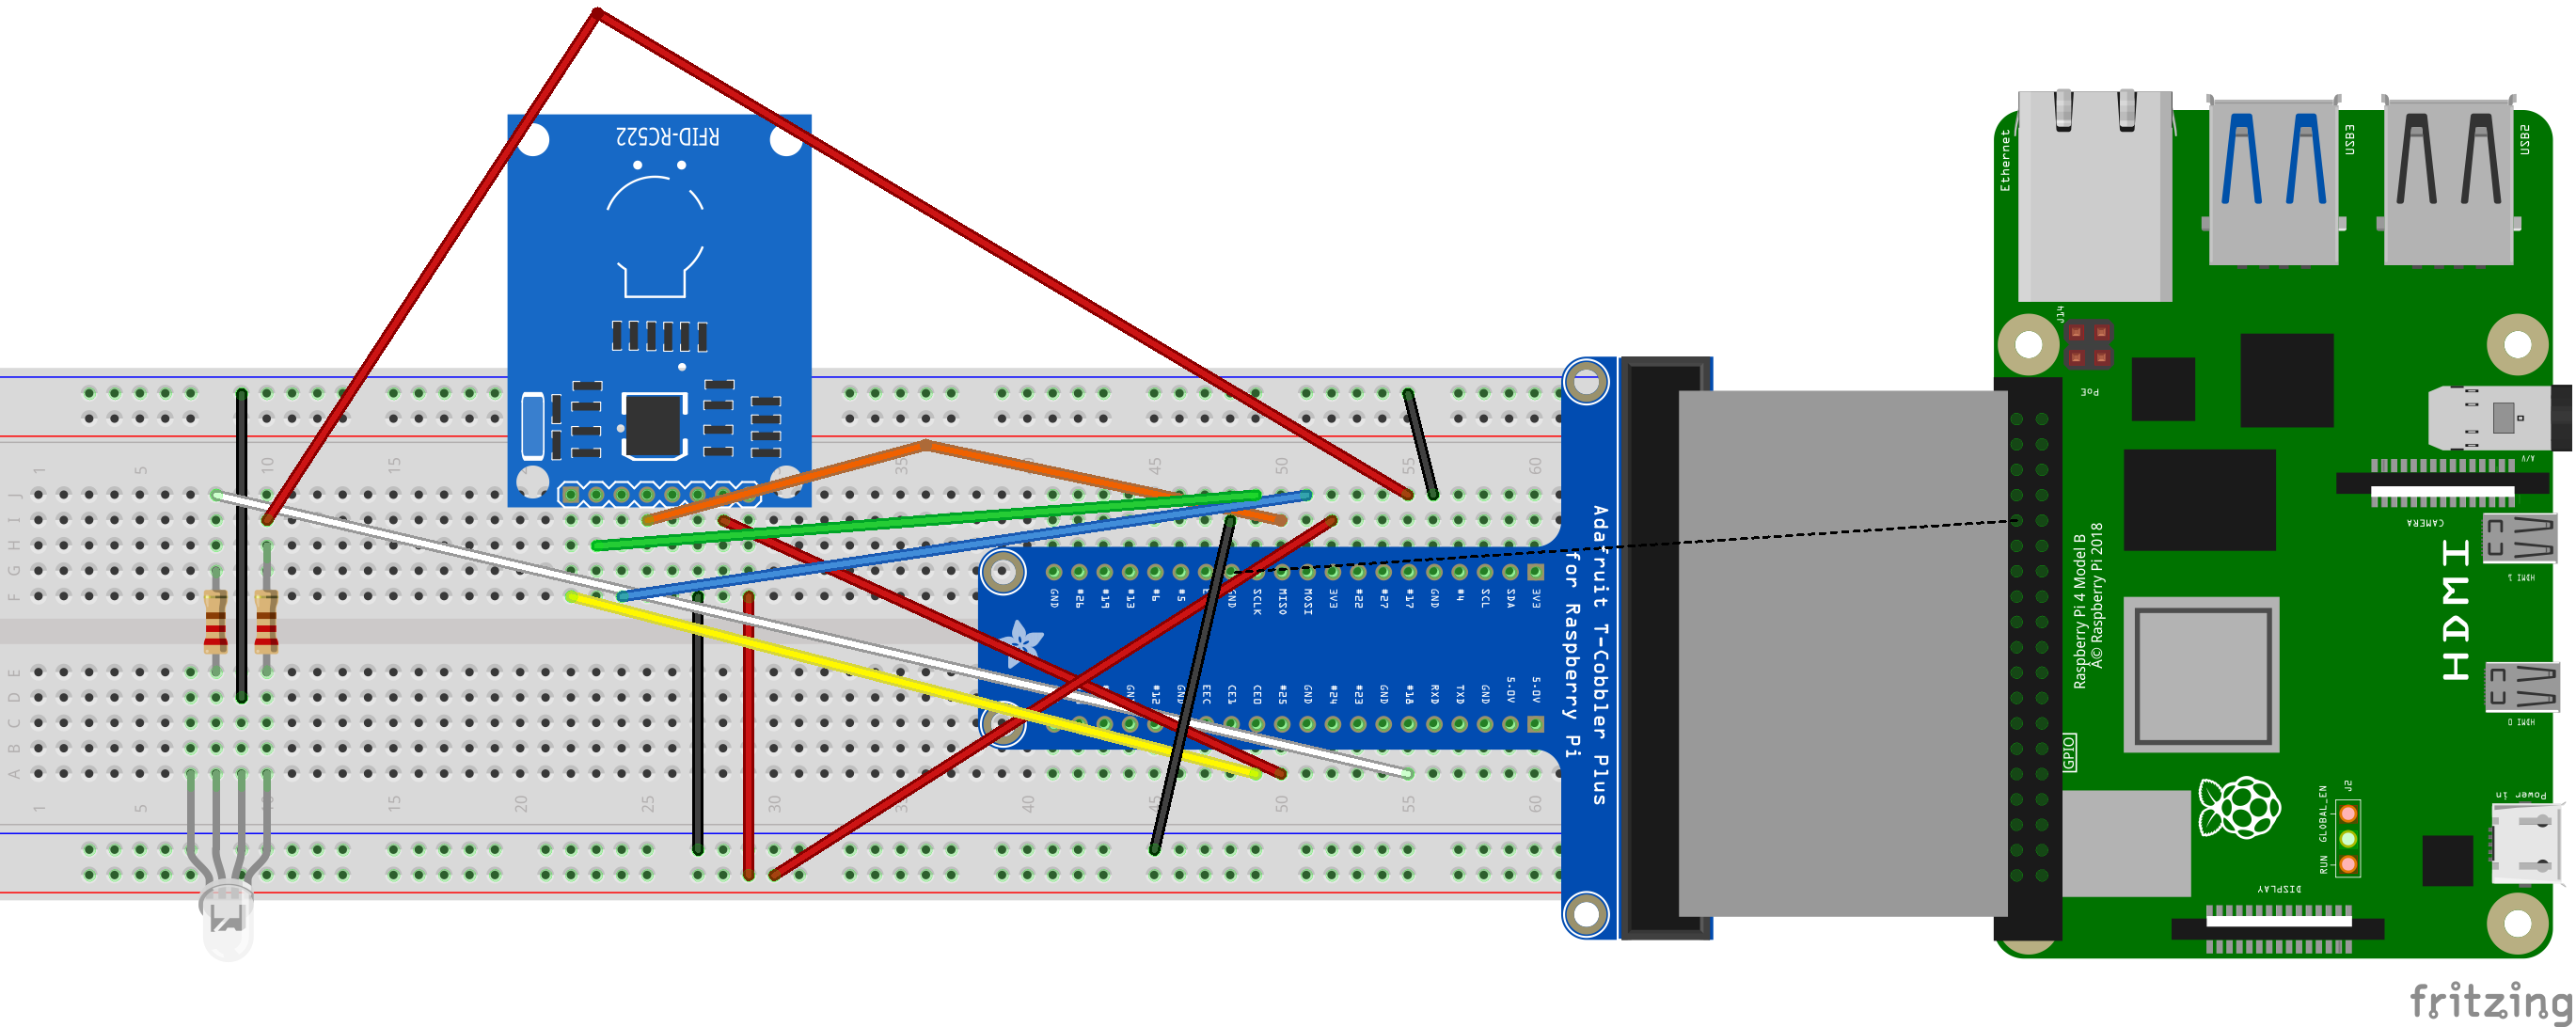
\includegraphics[width=\textwidth]{images/nfc-test-circuit.png}
\caption{Test Circuit for NFC Security Badge Reader}
\label{fig:nfc-test-circuit}
\end{figure}

\subsection{Electronic Door Lock}

The electronic door lock model will be powered by a servo motor. The chosen
servo motor is the Adafruit Micro Servo.  This servo has 180 degrees of motion
that can be traversed in 0.3 seconds.  The servo operates between 3V and 6V so
it can be powered through the Raspberry Pi's 5V line.

\begin{figure}[!htb]
\centering
\includegraphics{uml/electronic-lock-schematic.png}
\caption{Test Circuit for the Electronic Lock}
\label{fig:electronic-lock-schematic}
\end{figure}

\subsection{Time of Flight Range Sensor}

\begin{figure}[!htb]
\centering
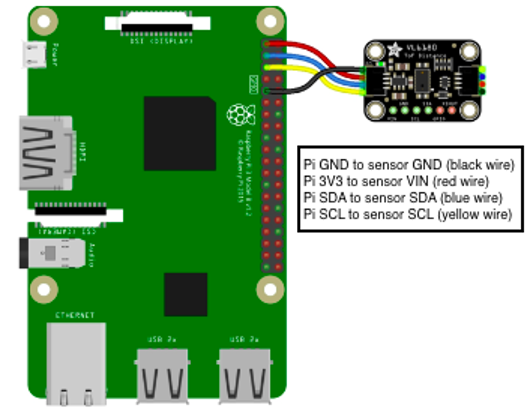
\includegraphics[width=0.6\textwidth]{images/tof-test-circuit.png}
\caption{Test Circuit for Time of Flight Sensor}
\label{fig:tof-test-circuit}
\end{figure}


\subsection{Control Server}

The control server hardware will consist of a Raspberry Pi connected to a
monitor, keyboard and mouse.

